\documentclass[titlepage]{article}

\usepackage[english]{babel}
\usepackage[utf8]{inputenc}
\usepackage{amsmath}
\usepackage{listings}
\usepackage{courier}
\usepackage{amsthm}
\usepackage{graphicx}
\usepackage[colorinlistoftodos]{todonotes}
\usepackage{amssymb}
\usepackage{mathtools}
\usepackage{listings}
\usepackage[inline]{enumitem}
\usepackage{tikz}
\usepackage{tabularx}
\usepackage{lstautogobble}
\usepackage{algorithm}
\usepackage{todonotes}
\usepackage[noend]{algpseudocode}
\usepackage[a4paper,left=3cm,right=3cm,top=3cm,bottom=3cm]{geometry}
\usepackage{titlesec}
\usepackage{siunitx}
\usepackage{mathrsfs}
\usepackage{setspace}
\usepackage{fixltx2e}
\usepackage{hyperref}
\usepackage{csquotes}
\usepackage{colortbl}
\usepackage{indentfirst}
\usepackage[T1]{fontenc}
\linespread{2}
\lstset{basicstyle=\footnotesize\ttfamily,breaklines=true,lineskip={-1pt}}
\titlelabel{\thetitle.\quad}
\allowdisplaybreaks
\delimitershortfall-1sp

\usetikzlibrary{arrows}
\usetikzlibrary{automata,positioning}

\title{Extend\\ Language Reference Manual}
\author{Ishaan Kolluri, Kevin Ye, Jared Samet, Nigel Schuster}
\date{\today}
\begin{document}
\maketitle
\tableofcontents
\section{Introduction to Extend}
	Extend is a domain-specific programming language used to designate ranges of cells as reusable functions. It abstracts dependencies between cells and models a dependency graph during compilation. In order to offer great performance for any size of datasets, Extend compiles down to LLVM.
	\newline
	Extend's syntax is meant to provide clear punctuation and easily understandable cell range access specifications, while maintaining the look of modern functional programming languages. Given Extend's functionality resonates well with spreadsheets, it borrows syntactical elements from programs such as Microsoft Excel.
\section{Structure of an Extend Program}
	Extend is predominantly composed of function declarations. In order to run the program, the \textbf{main} function will be executed. To illustrate the scope of the language, the OCaml grammar is attached below:
\lstinputlisting{./src/main/parser.mly}
\section{Types and Literals}
	\subsection{Primitive Data Types}
		Extend has two primitive data types, \textbf{numbers} and \textbf{ranges}. In the vein of Javascript, numbers are essentially 64-bit floating point numbers in Extend. Ranges are elaborated on in the next section. The user can choose to represent numbers in the following different ways:
		\newline
		\underline{\textbf{Char}}\newline
		A \textbf{char} literal is essentially a size 1 numerical range. At evaluation, the number in the range will be compared with its ASCII equivalent.
  		\newline
		\underline{\textbf{String}}\newline
  		A \textbf{string} literal is a range of numbers of size \textit{n}, where \textit{n} is the length of the string. The string 'hello' can be represented internally as [104, 101, 108, 108, 111].
		\newline
		\underline{\textbf{Integer}}\newline
		A \textbf{integer} can be represented as a size 1 numerical range as well. However, it retains its numerical value upon evaluation. 
		\newline
		\underline{\textbf{Float}}\newline
		A \textbf{float}, like Javascript numbers, can be represented as 64 bit, where the fraction is stored in bits 52 to 62.
		\newline
		Below is a snippet illustrating programmatic declarations for each of the above types.
  		\begin{lstlisting}
/* Integer */
num = 5;
/* Char */
chr = 'A'
/* String */
str = 'Hello'
/* Float */
num = 1.5;
  		\end{lstlisting}
	\subsection{Ranges}
		Ranges are a data type unique to the Extend language. It borrows conceptually from spreadsheets; a range is a group of cells with dimensions represented as rows and columns. Each range is either one or two-dimensional. A range is composed of cells, and cells are comprised of functions that can have dependencies on the values of other cells. 
		A range is written as follows:
		\begin{lstlisting}
/* This is a left-handed range, used to assign a value. */
[1,2]foo; /*Range with 1 row and 2 columns */
		\end{lstlisting}
		\subsubsection{Range Slicing}
			Extend somewhat mimics Python in its range slicing syntax; however, it offers the ability to slice a range in both absolute and relative terms.
			\begin{lstlisting}
foo[1,2] /* This evaluates to the cell value at row 1, column 2. */
foo[1,] /* Evaluates to the range of cells in row 1. */
foo[,2] /* Evaluates to the range of cells in column 2.*/
foo[,[1]] /* The internal brackets denote RELATIVE notation. 
In this case, 1 column right of the one currently being operated on. */ 
foo[5:, 7:] /* 5th row down, and 7th column from the absolute origin.
foo[[1:2], [5:7]] 
/* Selects the rows between the 1st and 2nd row from current row */
/* Selects the columns between 5th and 7th column from current column */
			\end{lstlisting}
		\subsubsection{The Underscore Symbol}
			The underscore(\_) symbol allows the dimension of the range to have an unspecified size. For example, in function signatures, using the underscore allows the return value to have various possible dimensions. An example is illustrated below:
			\begin{lstlisting}
[1,_]foo; 
/* A range with 1 row and an unknown, variable number of columns. */
			\end{lstlisting}

\section{Expressions}
\subsection{Operators}
\subsubsection{Multiplication}
\subsubsection{Addition}
\subsubsection{Unary}
\subsection{Booleans}
\subsection{Variable Declaration}
\subsection{Variable Assignment}
\subsection{Conditionals}
\section{Functions}
\label{sec:Functions}
Functions lie at Extend's core; however, they are not \textit{first class objects}. Since it can be verbose to write certain operations in Extend, the language will feature a small number of built-in functions and and a comprehensive standard library. An important set of built-in functions will handle I/O (see section~\ref{sec:IO}). Besides the built-in file I/O functions, all functions in Extend are free of side effects.
\subsection{Format}
\label{sec:funcdecl}
Every function in Extend follows the same format, but allows some optional declarations. As in most programming languages, the header of the function declares the parameters it accepts and the dimensions of the return value. The body of the function consists of an optional set of variable declarations and formula assignments, which can occur in any order, and a return statement, which must be the last statement in the function body. All variable declarations and formula assignments, in addition to the return statement, must be terminated by a semicolon.
This very simple function returns whatever value is passed into it:
\lstinputlisting{./samples/functions_simple.xtnd}
The leading \texttt{[1,1]} marks the return dimensions. \texttt{foo} is the function name. In parentheses the function arguments are declared, again with dimensions of the input. The body of the function follows, which in this case is only the return statement.
\subsection{Variable Declaration}
\label{sec:vardecl}
A variable declaration associates an identifier with a range of the specified dimensions, which are listed in square brackets before the identifier. For convenience, if the square brackets and dimensions are omitted, the identifier will be associated with a 1x1 range, and if only a single dimension is listed instead of two, the identifier will be associated with a range consisting of one row and the specified number of columns. In addition, multiple identifiers, separated by commas, can be listed after the dimensions; all of these identifiers will be separate ranges, but with equal dimension sizes. The dimensions can be specified either as literal integers or as expressions that evaluate to integers.
\begin{lstlisting}
[2, 5] foo; // Declares foo as a range with 2 rows and 5 columns
[m, n] bar; // Declares bar as a range with m rows and n columns
baz; // Declares baz as a 1x1 range
[10] ham, eggs, spam; // Declares ham, eggs and spam as distinct 1x10 ranges
\end{lstlisting}
\subsection{Formula Assignment}
\label{sec:formula}
A formula assignment assigns an expression to a subset of the cells of a variable. Unlike most imperative languages, this expression is not immediately evaluated, but is instead only evaluated if and when it is needed to calculate the return value of the function. A formula assignment consists of an identifier, an optional pair of slices enclosed in square brackets specifying the subset of the cells that the assignment applies to, an \texttt{=}, and an expression, followed by a semicolon. The slices specifying the cell subset can contain arbitrary expressions, as long as the expression taken as a whole evaluates to an integer.
\begin{lstlisting}
[5, 2] foo, bar;
foo[0,0] = 42; // Assigns the expression 42 to the first cell of the first row of foo
foo[0,1] = foo[0,0] * 2; // Assigns (foo[0,0] * 2) to the 2nd cell of the 1st row of foo
bar = 3.14159; // Assigns pi to every cell of every row of bar

/* The next line assigns foo[[-1],0] + 1 to every cell in
   both columns of foo, besides the first row */
foo[1:,0:1] = foo[[-1],0] + 2;
\end{lstlisting}
The last line of the source snippet above demonstrates the idiomatic Extend way of simulating an imperative language's loop; foo[4,0] would evaluate to 42+2+2+2+2 = 50 and foo[4,1] would evaluate to (42*2)+2+2+2+2 = 92. Although this may appear wasteful, intermediate values can be garbage collected once they are no longer needed to calculate the function's return value.
\subsubsection{Combined Variable Declaration and Formula Assignment}
For convenience, a variable declaration and a formula assignment to all cells of that variable can be combined on a single line by inserting a \texttt{:=} and an expression after the identifier. Multiple variables and assignments, separated by commas, can be declared on a single line as well.
\begin{lstlisting}
/* Creates two 2x2 ranges; every cell of foo evaluates to 1 and every cell of
   bar evaluates to 2. */
[2,2] foo := 1, bar := 2;
\end{lstlisting}
\subsubsection{Formula Assignment Errors}
If the developer writes code in such a way that more than one formula applies to a cell, this causes a compile-time error if the compiler can detect it or a runtime error if the compiler cannot detect it in advance and the cell is evaluated. If there is no formula assigned to a cell, the cell will evaluate to \texttt{empty}.
\subsection{Dimension Assignment}
\par Extend will feature gradual typing for function declarations. This will enable users with a weak experience in typing to use the language, while allowing more sophisticated developers to enforce type checking at compile time. In addition, it allows the developer to return ranges whose size is an unpredictable or complex function of the inputs.
\par To avoid specifying the precise return dimensions, an underscore can be used. This marks a variable range. Thus our function now looks like this:
\lstinputlisting{./samples/functions_dim_range_u.xtnd}
Here we are selecting a range from arg1 that depends on the value of arg2 and can therefore not be known ahead of time.
\subsection{Parameter Declarations}
If a parameter is declared with an identifier for the dimensions, instead of an integer literal, that identifier will contain the dimension size of the argument inside the function. In addition, expressions consisting solely of other identifiers are allowed, and will cause a run-time error if the sizes of the arguments are not consistent.
\par However Extend will feature even more options to specify ranges. If a certain operation should be applied to a range of numbers of unknown size, the size can be inferred at runtime and match the return size:
\lstinputlisting{./samples/functions_dim_range_v.xtnd}
This function will add 1 to each element in arg. Notice, that \texttt{m} is used across the function as a variable identifier to apply the operation to the range.
\par Summarizing, we have 3 ways of specifying a return range:\newline
\begin{tabularx}{\columnwidth}{| c | c | X |} \hline
Type & Symbol Example & Description \\ \hline
Number & 3 & A number is the simplest descriptor. It specifies the absolute return size \\ \hline
Expression & bar * 2 & An expression that can be anything, ranging from a simple arithmetic operation to a function call. To use this, any identifier used, must also be present as a range descriptor in a function parameter. \\ \hline
Underscore & \_ & This marker is unique, since it is a wildcard. While the other options aim to be specific, the underscore circumvents declaring the range size. \\ \hline
\end{tabularx}
\subsection{Application on Ranges}
Extend gives the developer the power to easily apply operations in a functional style on ranges. As outlined in the section above, there are various ways to apply functions to ranges. A feature unique to Extend is the powerful operation on values and ranges. To apply a function on a per cell basis, the corresponding variable needs to be preceded by "\#". The following function applies cell wise addition:
\lstinputlisting{./samples/functions_range_single.xtnd}
While both function above result in the same value, and only show the syntactical difference. If we wanted each cell to to be the square root divided by the sum of the input we have the following:
\lstinputlisting{./samples/functions_range_mix.xtnd}
Notice that \texttt{arg} is only once preceded by \texttt{\#}.
\subsection{Dependencies Illustrated}
The dependency resolution is another asset that sets Extend apart from other languages. Most languages compile ordinarily and execute the given commands sequentially. Extend builds a dependency graph. The advantage of this is that only relevant code segments will be executed. Given the function
\lstinputlisting{./samples/functions_dep_graph.xtnd}
The dependency graph will look like this: \newline
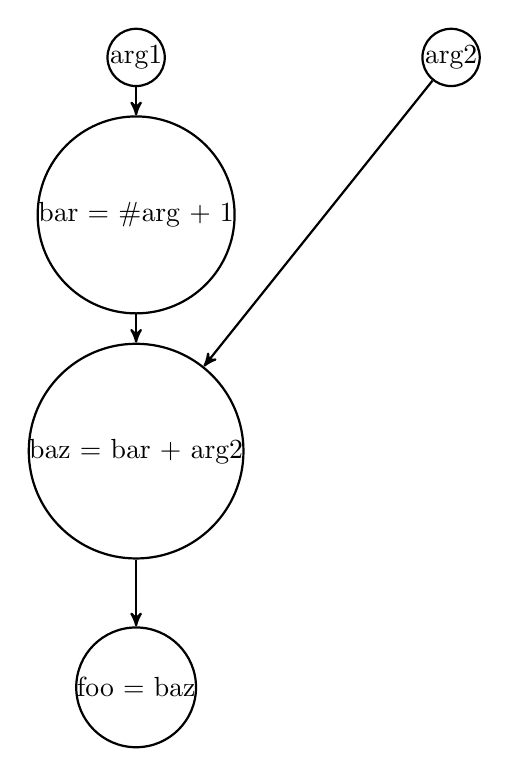
\begin{tikzpicture}[->,>=stealth',shorten >=0pt,auto,node distance=3cm,
        thick,main/.style={circle,draw,minimum size=0.6cm,inner sep=0pt]}]
		\node [main] (1) at (0, 2) {arg1};
		\node [main] (2) at (4, 2) {arg2};
		\node [main] (3) at (0, 0) {bar = \#arg + 1};
		\node [main] (4) at (0, -3) {baz = bar + arg2};
		\node [main] (5) at (0, -6) {foo = baz};
		\draw (1) to (3);
		\draw (3) to (4);
		\draw (4) to (5);
		\draw (2) to (4);
\end{tikzpicture} \newline
Notice that \texttt{faz} does not appear in the graph, because it is not relevant for the return value. Ultimately this graph enables Extend to find the leaves, evaluate code paths in the best configuration and even in parallel.

\section{File I/O}
\label{sec:IO}
Although the anticipated use cases of Extend generally do not include highly interactive programs, the language allows the developer to read from and write to files, including stdin, stdout, and stderr.
\subsection{File Pointers}
\subsection{Reading and Writing}
\subsection{Input Arguments}
\subsubsection{How to run a program}
\subsubsection{Main function}

\section{Entry Point, External Libraries, Scoping and Namespace}
\subsection{\texttt{main} function}
When a compiled Extend program is executed, the \texttt{main} function is evaluated. All computations necessary to calculate the return value of the function are performed, after which the program terminates. The \texttt{main} function must be a function of a single argument, conventionally denoted args, which is guaranteed to be a 1-by-n range containing the command line arguments.
\subsection{Scoping and Namespace}
There is a single namespace for functions and global variables that is shared between all files composing an Extend program. As a result, multiple definitions of functions with the same name, whether in the same file or not, will cause a compile-time error. However, functions may declare local variables sharing a name with a global variable; the local variable defintion will override the global variable within that function. Function definitions may not be nested. If an outer function passes a variable into an inner function call, lazy evaluation may mean that the inner function indirectly has access to variables defined in the outer function call; however, 

\subsection{External Libraries}

\label{sec:ExternFunctionSignatures}

\section{Example Program}
\lstinputlisting{./samples/sequence.xtnd}

\end{document}
